\documentclass[urlcolor=blue,dvipsnames]{beamer}

\usepackage[utf8]{inputenc}
\usepackage{fancybox,fancyvrb}
\usepackage{environ,xspace,empheq}

\usepackage{tikz}
\usetikzlibrary{arrows.meta,decorations.markings,decorations.pathreplacing,fadings,positioning}

\hypersetup{colorlinks,linkcolor=,urlcolor=cyan}

\beamertemplatenavigationsymbolsempty
\setbeamertemplate{footline}[frame number]
\usetheme{Pittsburgh}

%\makeatletter
%\newcommand{\tinytiny}{\@setfontsize{\tinytiny}{4pt}{4pt}}
%\makeatother

\newcommand\enumnum[1]{{\renewcommand{\insertenumlabel}{#1}%
      \usebeamertemplate{enumerate item} \,}}

\newcommand{\grad}{\nabla}
\newcommand{\ih}{\boldsymbol{\hat{\textbf{\i}}}}
\newcommand{\jh}{\boldsymbol{\hat{\textbf{\j}}}}
\newcommand{\vF}{\boldsymbol{\vec{\textbf{F}}}}
\newcommand{\Matlab}{\textsc{Matlab}\xspace}
\newcommand{\Octave}{\textsc{Octave}\xspace}


\title{7.4 Laplace Transforms: \\ convolutions}

\subtitle{a lesson for MATH F302 Differential Equations}

\author{Ed Bueler, Dept.~of Mathematics and Statistics, UAF}

\date{\tiny \today}


\begin{document}
\setbeamertemplate{itemize item}{$\bullet$}
\setbeamertemplate{itemize subitem}{$\circ$}
\renewcommand{\thefootnote}{{\color{green} \arabic{footnote}}}

\begin{frame}
\titlepage

\centerline{\tiny for textbook: \, D. Zill, \emph{A First Course in Differential Equations with Modeling Applications}, 11th ed.}
%\color{green!40!blue}
\end{frame}

\newcommand{\LL}[1]{\mathcal{L}\left\{#1\right\}}
\newcommand{\LLi}[1]{\mathcal{L}^{-1}\left\{#1\right\}}


\begin{frame}{the transfer function}

\begin{itemize}
\item consider a damped mass-spring system with driving force $g(t)$:
\begin{equation}
m x'' + \beta x' + k x = g(t), \qquad x(0)=0, \, x'(0)=0  \tag{$\ast$} \label{drivenmassspring}
\end{equation}
\item applying $\mathcal{L}$ we get, after simplifying,
    $$X(s) = \frac{1}{ms^2+\beta s+k}\,G(s)$$
\item the function
    $$\alert{F(s) = \frac{1}{ms^2+\beta s+k}}$$
is the \alert{\emph{transfer function}} of \eqref{drivenmassspring}
\item \emph{so}: the Laplace transform of $x(t)$ is simply the product of the transfer function and the transformed driving force:
    $$X(s) = F(s) G(s)$$
\end{itemize}
\end{frame}


\begin{frame}{remember the table?}

\vspace{-5mm}
\begin{center}
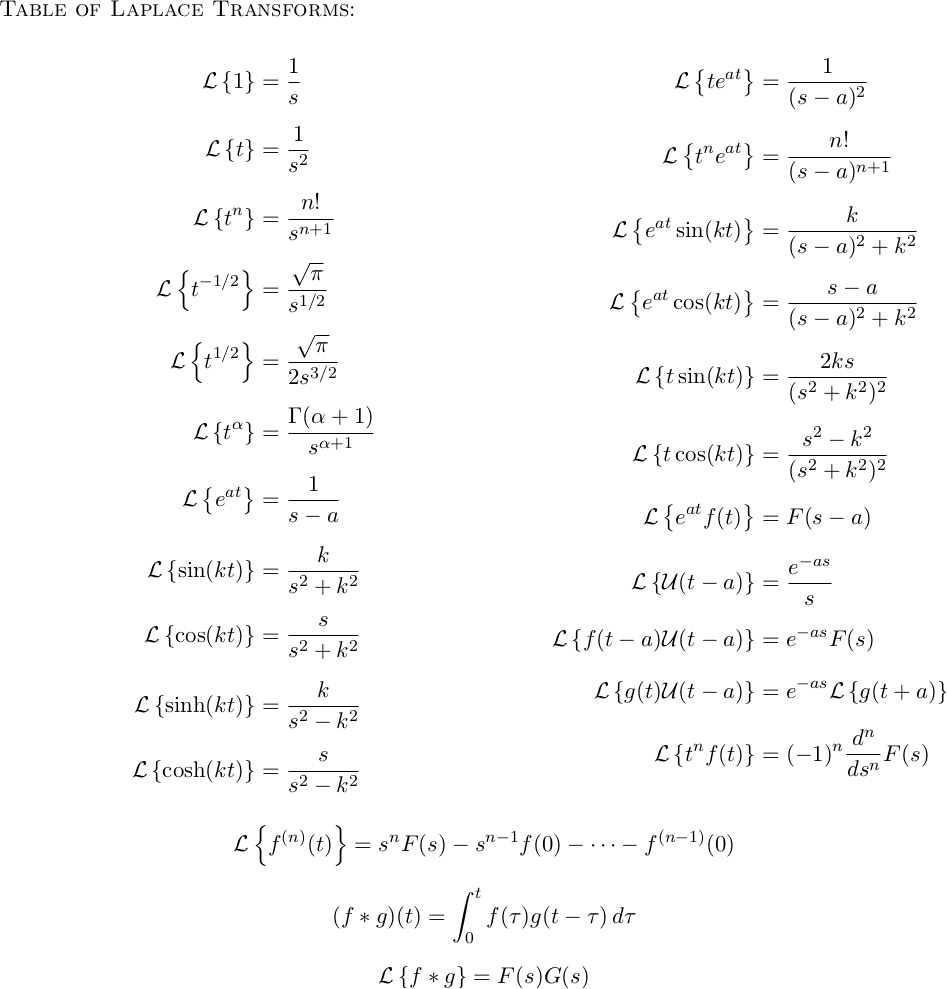
\includegraphics[height=80mm]{figs/fulllaplacetable}
\end{center}

\vspace{-13mm}
\alert{\emph{note last two entries $\to$}}
\end{frame}


\begin{frame}{convolution}

the last two entries say:

\bigskip
\begin{itemize}
\item \emph{definition.}  given functions $f(t)$ and $g(t)$ defined on $(0,\infty)$, the function
    $$\alert{(f \ast g)(t) = \int_0^t f(\tau) g(t-\tau)\,d\tau}$$
is called the \alert{\emph{convolution}} of $f$ and $g$
\item \emph{the convolution theorem.}  if $F(s)=\LL{f(t)}$ and $G(s)=\LL{g(t)}$ then
    $$\alert{\LL{f \ast g} = F(s) G(s)}$$
\end{itemize}
\end{frame}


\begin{frame}{why the convolution matters}

\begin{equation}
m x'' + \beta x' + k x = g(t), \qquad x(0)=0, \, x'(0)=0 \label{dms} \tag{$\ast$}
\end{equation}
     $$\alert{X(s) = F(s) G(s)} \quad \text{ where } \quad \alert{F(s) = \frac{1}{ms^2+\beta s+k}}$$

\begin{itemize}
\item let $f(t)=\LLi{F(s)}$
    \begin{itemize}
    \item the \emph{impulse response} or \emph{weight function} of problem \eqref{dms}
    \end{itemize}
\item by the convolution theorem,
    $$\alert{x(t) = (f * g)(t)}$$

\vspace{-2mm}
    \begin{itemize}
    \item the solution comes from \emph{convolving} the impulse response and the driving force
    \end{itemize}
\end{itemize}
\end{frame}


\begin{frame}{warning: convolution vs.~multiplication}

\begin{itemize}
\item the Laplace transform of a product of function is \alert{\emph{NOT}} the product of Laplace transforms
    $$\LL{f(t)\, g(t)} \neq F(s) G(s)$$

\vspace{-3mm}
    \begin{itemize}
    \item why not?
    \end{itemize}

\bigskip\bigskip\bigskip

\item \emph{convolution} on the $t$ side becomes multiplication on the $s$ side:
    $$\LL{f(t)\ast g(t)} = F(s) G(s)$$
\item i.e.
    $$\LL{f\ast g} = \LL{f} \LL{g}$$
\end{itemize}
\end{frame}


\begin{frame}{computing convolution: example 1}

\begin{itemize}
\item definition: \qquad $(f \ast g)(t) = \int_0^t f(\tau) g(t-\tau)\,d\tau$
\item \emph{example 1.} compute $f\ast g$:
  $$f(t) = 1-\mathcal{U}(t-2) = \begin{cases} 1, & 0\le t < 2 \\ 0, & t\ge 2 \end{cases}, \qquad g(t) = e^{-t}$$
\end{itemize}

\vspace{45mm}
\end{frame}


\begin{frame}{computing convolution: example 2}

\begin{itemize}
\item \emph{example 2.} compute $f\ast g$:
  $$f(t) = \sin(t), \qquad g(t) = e^{-t} \hspace{50mm}$$
\end{itemize}

\vspace{60mm}
\end{frame}


\begin{frame}{but what does a convolution \emph{look} like?}

\begin{itemize}
\only<1>{\item[ex.~1:] {\color{blue} $f(t)=1-\mathcal{U}(t-2)$} and {\color{red} $g(t)=e^{-t}$}}
\only<2>{\item {\color{blue} $f(t)=\mathcal{U}(t-2)-\mathcal{U}(t-4)$} and {\color{red} $g(t)=e^{-t}$}}
\only<3>{\item[ex.~2:] {\color{blue} $f(t)=\sin(t)$} and {\color{red} $g(t)=e^{-t}$}}
\only<4>{\item {\color{blue} $f(t)=\sin(\pi t)$} and {\color{red} $g(t)=e^{-t}$}}
\end{itemize}

\begin{center}
\includegraphics<1>[width=0.7\textwidth]{figs/convolution1}
\includegraphics<2>[width=0.7\textwidth]{figs/convolution2}
\includegraphics<3>[width=0.7\textwidth]{figs/convolution3}
\includegraphics<4>[width=0.7\textwidth]{figs/convolution4}
\end{center}
\end{frame}


\begin{frame}{convolutions are a big deal}

instead of trying to show you here, go to:
\begin{center}
\href{https://en.wikipedia.org/wiki/Convolution}{\texttt{en.wikipedia.org/wiki/Convolution}}
\end{center}

\begin{itemize}
\item images and movies of 1D convolutions
\item discrete 1D convolution is a \emph{filter} in signal processing
\item discrete 2D convolution is a \emph{filter} in image processing
\end{itemize}
\end{frame}


\begin{frame}{exercise \S7.4 \#19}

\begin{itemize}
\item \emph{example 3.}  find the convolution $f\ast g$ of the functions, and then find the Laplace transform of the result:
    $$f(t)=4t, \qquad g(t)=3t^2 \hspace{50mm}$$
\end{itemize}

\vspace{50mm}
\end{frame}


\begin{frame}{exercise \S7.4 \#26}

\begin{itemize}
\item convolution theorem: \quad $\LL{f \ast g} = F(s) G(s)$
\item \emph{example 4.}  find the Laplace transform of $f\ast g$ using the convolution theorem; do not evaluate the convolution integral before transforming:
    $$f(t)=e^{2t}, \qquad g(t)=\sin(t) \hspace{50mm}$$
\end{itemize}

\vspace{40mm}
\end{frame}


\begin{frame}{exercise \S7.4 \#28}

\begin{itemize}
\item the convolution of $f(t)$ with the constant 1 is just the integral:
    $$f(t) \ast 1 = \int_0^t f(\tau) 1\,d\tau = \int_0^t f(\tau)\,d\tau$$
\item so
    $$\LL{\int_0^t f(\tau)\,d\tau} = \LL{f(t)\ast 1} = \frac{F(s)}{s}$$
\item \emph{example 5.}  compute the Laplace transform:
    $$\LL{\int_0^t \cos \tau\,d\tau} = \hspace{50mm}$$
\end{itemize}

\vspace{25mm}
\end{frame}


\begin{frame}{like exercise \S7.4 \#35}

\begin{itemize}
\item \emph{example 6.}  compute the inverse Laplace transform:
    $$\LLi{\frac{1}{s(s-3)}} = \hspace{80mm}$$

\vspace{40mm}
\hfill \scriptsize \emph{what was the old way?}
\end{itemize}
\end{frame}


\begin{frame}{the main idea (\emph{a summary})}

for a damped mass-spring system with driving force $g(t)$,
\begin{equation*}
m x'' + \beta x' + k x = g(t), \qquad x(0)=0, \, x'(0)=0
\end{equation*}

\begin{enumerate}
\item the \emph{transfer function}
    $$F(s) = \frac{1}{ms^2+\beta s+k}$$
is multiplied by the transformed driving force to give the Laplace transform of the solution $x(t)$:
    $$X(s) = F(s) G(s)$$
\item $f(t)=\LLi{F(s)}$ is \emph{impulse response} of mass-spring system
\item solution is convolution of impulse response and driving force:
    $$x(t) = (f * g)(t)$$
\end{enumerate}
\end{frame}


\begin{frame}{why ``impulse response''?}
\begin{itemize}
\item X
\end{itemize}
\end{frame}

\begin{frame}{$\Gamma$ function}
\begin{itemize}
\item X
\end{itemize}
\end{frame}


\begin{frame}{expectations}

\begin{itemize}
\item just watching this video is \emph{not} enough!
     \begin{itemize}
     \item see ``found online'' videos and stuff at

     \centerline{\href{https://bueler.github.io/math302/week11.html}{\tt \color{cyan} bueler.github.io/math302/week11.html}}
     \item \emph{read} ``7.4.2 Transforms of Integrals'' in \S7.4
     \item \emph{do} the WebAssign exercises for section 7.4
     \end{itemize}
\end{itemize}
\end{frame}

\end{document}

